% !TEX program = lualatex

\documentclass[
11pt,
captions=tableheading,
smallheadings,
%headings=big,
headsepline,
footsepline, 
%chapterprefix=false			% weiss nicht was passiert
parskip=half-,
%BCOR=10mm,
%twocolumn, 
%draft
]{scrartcl}

%\usepackage[babelshorthands]{polyglossia}
\usepackage{polyglossia}
%\setdefaultlanguage[variant = swiss]{german}
\setdefaultlanguage{german}

%\usepackage[ngerman]{babel} 
\usepackage[]{ scrlayer-scrpage }
\usepackage[ a4paper,
 total={165mm,250mm},
 left=25mm,
 top=25mm,
 headsep=10mm
 %footsep=12mm
 %,showframe
  ]{geometry}
 \usepackage{fontspec}
\setmainfont{Times New Roman}
\setsansfont{Arial}

\usepackage[dvipsnames]{xcolor}
\usepackage{forest}
\usepackage[most]{tcolorbox}
\usepackage[
version=3,
arrows=pgf-filled,
]{mhchem} % für chemische Formeln
\usepackage{microtype}
\usepackage{float}
\usepackage{enumitem}
\usepackage{multicol}
\usepackage{booktabs}
\usepackage{tabularx}
\usepackage{longtable}
\usepackage{fontawesome5}
\usepackage{pdfpages}
\usepackage{pgfgantt}
\usepackage{enumitem}
\setlist{noitemsep} % Entfernt den zusätzlichen Abstand zwischen Listenelementen

\usepackage{tikz}
\usetikzlibrary{shapes.geometric, arrows}

\tikzstyle{arrow} = [thick,->,>=stealth]
\tikzstyle{block} = [align=center]


\usepackage{pdflscape} % Für Querformat-Seiten


\usepackage{siunitx}
\usepackage{amsfonts}
\usepackage{tabularx}

%Quellen 
\usepackage[
    backend=bibtex, 
    natbib=true,
    style=numeric,
    sorting=none
]{biblatex}
\addbibresource{../Quellen.bib}

\usepackage[section]{placeins} % avoids images in the wrong section


\usetikzlibrary{shapes.symbols, positioning, decorations.pathreplacing}

% order of hyperref, cleverref is important
\usepackage[hidelinks]{hyperref}
\usepackage{cleveref}



\frenchspacing



\floatplacement{figure}{H}

% Labeling of elements
\counterwithin{figure}{section}
\counterwithin{table}{section}
\counterwithin{equation}{section}

% Colors
\definecolor{blau_bauschule}{RGB}{22,65,148}

% Titel mit Bauschule blau gemäss CI manual
\addtokomafont{section}{\color{blau_bauschule}\Huge}
\addtokomafont{subsection}{\color{blau_bauschule}\huge}
\addtokomafont{subsubsection}{\color{blau_bauschule}\Large}
\addtokomafont{paragraph}{\normalsize}
\addtokomafont{subparagraph}{\small}
% Pagestyle
\pagestyle{scrheadings}
\ihead{\fontsize{9pt}{2pt}\selectfont }
\ohead{\fontsize{9pt}{2pt}\selectfont Baustoffe}
\chead{\fontsize{9pt}{2pt}\selectfont \headmark}
\ifoot{\fontsize{9pt}{2pt}\selectfont Bauschule Aarau} 
\ofoot{\fontsize{9pt}{2pt}\selectfont \thepage} %Seitennummer
\cfoot{\fontsize{9pt}{2pt}\selectfont }
\setkomafont{pagehead}{\normalfont}
\setkomafont{pagefoot}{\normalfont}
\setkomafont{pagefoot}{\normalfont}
\setkomafont{pagehead}{\normalfont}
\setkomafont{pagefoot}{\normalfont}
\setcounter{topnumber}{1}
\setcounter{bottomnumber}{1}
\automark[section]{subsection}


% Bild- und Tabellenunterschriften
\renewcommand*{\figurename}{Abbildung}
\renewcommand*{\tablename}{Tabelle}


% Titel
\title{Baustoffe}
%\author{Patrick Pfändler}
\date{2021}

% https://tex.stackexchange.com/questions/501018/how-to-write-a-minitoc-with-plain-koma-script

%https://www.mrunix.de/forums/archive/index.php/t-74962.html



%TODO % Studierende haben häufig eine Familie (noch integrieren) 


\makeatletter
\newcommand\reaction@[1]{\begin{equation}\ce{#1}\end{equation}}
\newcommand\reaction@nonumber[1]%
{\begin{equation*}\ce{#1}\end{equation*}}
\newcommand\reaction{\@ifstar{\reaction@nonumber}{ \reaction@}}
\makeatother
%renewtagform{reaction}[R ]{(}{)}

%% Custom icons 
\newcommand{\Lernziel}{\faBullseye}
\newcommand{\Diskussion}{\faComments}
\newcommand{\TR}{\faCalculator}
\newcommand{\Fragen}{\faQuestionCircle}
\newcommand{\LeherTafel}{\faChalkboardTeacher}

\forestset{
    folder/.style={
        for tree={
            grow=east,
            rectangle,
            draw,
            rounded corners,
            align=center,
            fill=blue!20,
            text width=4.5cm, % Breitere Blöcke
            minimum height=1cm,
            font=\footnotesize % Kleinere Schriftgrösse
        }
    },
    document/.style={
        for tree={
            grow=east,
            rectangle,
            draw,
            rounded corners,
            align=center,
            fill=gray!20,
            text width=4cm, % Breitere Dokumentenblöcke
            minimum height=0.8cm,
            font=\scriptsize % Kleinere Schriftgrösse
        }
    }
}







\begin{document}


\pagestyle{scrheadings}




%\renewcommand{\familydefault}{\sfdefault}
%\setkomafont{captionlabel}{\itshape \fontsize{10pt}{2pt}}
%\setkomafont{caption}{\sffamily} 



%\maketitle
{\color{blau_bauschule}\fontsize{40pt}{21pt}\selectfont \textbf{Lehrkonzept für die Lehrveranstaltung "Baustoffe"}}

\vspace{3cm}

{\color{blau_bauschule}\fontsize{31pt}{30pt}\selectfont \textbf{Abschlussarbeit im Fachkurs für Lehrpersonen HF mit integriertem SVEB~1}}

\vspace{2cm}

{\color{blau_bauschule}\fontsize{25pt}{25pt}\selectfont \textbf{
Ort: Bauschule Aarau \\
\vspace{0.4cm}
Coach: Natalie Raeber\\
\vspace{0.4cm}
Teilnehmer: Dr. Patrick Pfändler\\
\vspace{0.4cm}
Abgabedatum: 31.03.2025
\vspace{0.4cm}
}}
\vspace{1cm}





\clearpage
\setcounter{tocdepth}{3} % Tiefe des Inhaltverzeichnisses steuern
\tableofcontents%
\clearpage

\subsection*{Abkürzungsverzeichnis}
\begin{table}[H]
    \centering
    \label{tab:abkuerzungen}
    \begin{tabularx}{\textwidth}{@{}ll@{}}
        \toprule
        %\midrule
        Bsp. & Beispiel                \\
        LP   & Lehrperson              \\
        SF   & Sozialform              \\
        FK   & Fachkompetenz           \\
        ÜK   & Überfachliche Kompetenz \\
        IV   & Invalidenversicherung \\
        BSA & Bauschule Aarau AG \\
        \bottomrule
    \end{tabularx}
\end{table}



\clearpage
\section{Analyse der Vorraussetzungen}
Im nachfolgenden Abschnitt werden zunächst die wichtigsten Rahmenbedingungen zum Lehrkonzept im Fach Baustoffe erläutert und die Zielgruppe näher betrachtet. Die daraus gewonnen Einblicke bilden schliesslich die Grundlage für alle didaktischen Entscheidungen innerhalb des Lehrkonzepts (siehe \Cref{sec:Lernziele}).

\subsection{Rahmenbedingungen}
Die im Rahmen des vorliegenden Lehrkonzepts entwickelten Lektionen werden physisch in der Schweizerischen Bauschule Aarau AG (BSA), Suhrenmattstrasse 48, 5035 Unterentfelden durchgeführt.

\subsubsection{Räumliche und zeitliche Rahmenbedingungen}
Die zur Verfügung stehenden räumlichen Ressourcen beinhalten einen für das Fach fest zugeteilten Unterrichtsraum, mit drei Sitzreihen à sechs Stühlen und einem frontal platzierten Lehrpult. Der Raum umfasst damit eine Kapazität von 18 Studierenden. Die Sitzplätze im Unterrichtsraum sind fix zugeteilt. 

Um den Einsatz verschiedener Unterrichtsmethoden zu gewährleisten ist der Unterrichtsraum mit zwei fest installierten Decken-Beamern ausgestattet, einem Hellraumprojektor, einer Flipchart und frei verfügbarem W-LAN, was den Einsatz interaktiver Onlinetools während der Unterrichtslektion zulässt. 

Das Fach Baustoffe umfasst gemäss Planung insgesamt etwa 100 Unterrichtsstunden, die über ein Schuljahr verteilt sind. Der Unterricht wird in Blöcken von 90 bis 120 Minuten durchgeführt und erstreckt sich über rund 34 Schulwochen. Die Einheiten finden in der Regel am Montag oder Dienstag statt.

Insgesamt umfasst das vorliegende Lehrkonzept 8 Lektionen. Eine Lektion besteht aus 1 Stunde und 45 Minuten, welche auch die Abdeckung von Pausen beinhaltet. Die Lektion findet immer montags, von 15:15 Uhr bis 17:00 Uhr statt.

Der Unterricht selbst ist in der Regel Kontaktunterricht, wobei auch Phasen des selbständigen Arbeitens vorgesehen sind (siehe \Cref{sssec:ZeitlicheEinteilungLK}).

Während der o. g. 8 Lektionen ist mit einer Teilnahme von 14 Studierenden zu rechnen, welche für das Fach Baustoffe eingeschrieben sind. Diese 14 Studierenden befinden sich am Anfang ihrer Ausbildung zum Bauführer bzw. zur Bauführerin und sind zum Zeitpunkt der Durchführung des vorliegenden Lehrkonzepts im 2. Von insgesamt 6 Semestern. 

\subsubsection{Weitere Rahmenbedingungen}

Weitere Ressourcen, die im Fach Baustoffe genutzt werden können, sind die schuleigene Bibliothek. Zudem stehen für praktische Übungen und Demonstrationen weitere Flächen innerhalb des Gebäudes zur Verfügung. Neben der Bibliothek haben die Studierenden Zugang im Beisein der Lehrperson (LP) Zugang zur Materialsammlung der Bauschule Aarau, welche für die Ausgestaltung des vorliegenden Lehrkonzeptes relevant sein könnte. So befinden sich in den Schaukästen im Gebäude der BSA diverse Sammlungen von Baustoffen, wie beispielweise zu den Natursteinen.

Die Studierenden haben neben dem physischen Austausch vor Ort auch virtuellen Zugang zu der Applikation MS Teams. In diesem Tool können die Lehrunterlagen, praktische Übungen und aufkommende Fragen geteilt werden. MS Teams Channel wird von der LP vorbereitet und verwaltet (siehe \Cref{sssec:MS_Teams_LMS}). 

Der Unterricht selbst ist in der Regel Kontaktunterricht, wobei auch Phasen des selbständigen Arbeitens (z.B. Diplomarbeit) und der Gruppenarbeit vorgesehen sind. Das vorliegende Lehrkonzept bildet eine fundierte Vorbereitung auf die eidgenössische Prüfung zum Bauführer bzw. zur Bauführerin.

\subsubsection{Grundlangen für das Lehrkonzept}

Das Lehrkonzept baut auf den vorausgegangenen Lehrveranstaltungen in den Fächern Physik und Chemie auf und dient dem Fach Kunststoffe als Grundlange.
Als Nachweis der erworbenen Kompetenzen im Fach Baustoffe sind 6 Prüfungen geplant. 
Gemäss dem  dem Lehrplan der BSA im Laufe des Semesters mindestens 2 Prüfungen durchgeführt werden.

In den Prüfungen sollen die Fähigkeiten und Kompetenzen, welche die Studierenden u. a. aus dem vorliegenden Lehrkonzept erworben haben, abgefragt und überprüft werden. Diese Fähigkeiten und Kompetenzen sind ausgerichtet an dem Berufspädagogischen Konzept der BSA \cite{BerufspädagogischesKonzept_BauschuleAarau}, dem Lehrplan der BSA und dem Kompetenzprofil für BauführerInnen \cite{Kompetenzprofil_Baufuehrer}. Nach Erstellung und Durchführung des Lehrkonzepts sollen die Studierenden entsprechen über folgende Fähigkeiten und Kompetenzen verfügen:

\begin{itemize}
    \item Kenntnisse in grundlegender und spezialisierter Materialkunde
    \item Kenntnisse der Materialprüfung 
    \item  ökologische und wirtschaftliche Aspekte der Baustoffwahl
\end{itemize}


Das Kompetenzprofil für BauführerInnen schreibt konkret, dass
\begin{itemize}
    \item BauführerInnen veranlassen und koordinieren den Einsatz neuer Methoden, Technologien und Baustoffe. Sie sorgen dafür, dass neue Methoden, Technologien und Baustoffe auf Baustellen fachgerecht, zum richtigen Zeitpunkt und wirtschaftlich eingesetzt werden.
    \item Sie kontrollieren und überprüfen die Qualität der Baustoffe regelmässig entsprechend den Vorgaben. Dabei werden als kritische Erfolgsfaktoren die folgenden Punkte genannt:
    \begin{itemize}
        \item Gute Kenntnisse hinsichtlich multifunktionaler und intelligenter Baustoffe (einschliesslich Einsatz im Baubereich)
        \item Interesse an neuen Methoden, Technologien und Baustoffen (multifunktionale und intelligente Baustoffe (einschliesslich Einsatz im Baubereich) usw.) instruieren und anleiten können
    \end{itemize}
\end{itemize}

Neben diesen Fachkompetenzen (FK) sind auch die überfachlichen Kompetenzen (ÜK) von für die angehenden Bauführer und Bauführerinnen von grosser Bedeutung. So ist z. B. die Sozialkompetenz wichtig, um sich auf der Baustelle kompetent in neuen Teams einzufinden und effiziente Teamarbeit leisten zu können. Auch hier will das vorliegende Lehrkonzept zum Kompetenzerwerb beitragen, in dem diesbezüglich didaktisch geeignete Mittel zielführend gewählt und eingesetzt werden. 


\subsection{Zielgruppe}
Die Zielgruppe, welche dem vorliegenden Lehrkonzept zugrunde liegt, besteht aus angehenden Bauführern und Bauführerinnen im ersten und zweiten  von  insgesamt 6 Semestern. Die Studierenden sind zwischen 20 und 30 Jahre alt und haben meist eine Berufslehre als Maurer und zum Teil eine Weiterbildung zum Polier oder Vorarbeiter (inkl. Berufsbildnerkurs) abgeschlossen. 
Die Studierenden bringen unterschiedliche Vorkenntnisse und Erfahrungen mit, da sie aus verschiedenen beruflichen Hintergründen stammen (z. B. Maurer, Poliere, Quereinsteiger). Damit ist die Zielgruppe in der Erwachsenenbildung anzusiedeln. In die Zielgruppe eingeschlossen sind auch ältere Studierenden, welche aufgrund gesundheitlicher Einschränkungen von der Invalidenversicherung (IV) an die BSA überwiesen wurden, um dort die Ausbildung zum Bauführer zu absolvieren. Aus diesen Gründen lässt sich bei der Zielgruppe sowohl eine intrinsische, als auch eine extrinsische Motivation vorfinden. 
Wichtig ist auch, dass die Zielgruppe bereits über praktische Erfahrung im Baugewerbe verfügt und erste Erfahrungen in der Bauführung in Unternehmen gesammelt hat. 

Die Vorkenntnisse der Zielgruppe sind aufgrund der zuvor erworbenen bzw. nicht erworbenen Weiterbildungen sehr variabel. Ebenfalls besteht eine grosse Heterogenität in den Lernvoraussetzungen, da die Studierenden aus unterschiedlichen Berufsfeldern (Stichwort: Quereinsteiger) kommen.

Bei der Zielgruppe ist herauszustellen, dass die Studierenden aufgrund ihres eher fortgeschrittenen Alters gerade zu Beginn der schulischen Ausbildung das lange Sitzen im Unterricht nicht gewöhnt sind.

Im Hinblick auf die Kenntnisse in der Anwendung von digitalen, kollaborativen Tools sind innerhalb der Zielgruppe unterschiedlich Ausprägungen vorhanden. Je nach Ausbildungsstand ist auch die Selbstorganisation der Studierenden unterschiedlich ausgeprägt. Die Mehrheit der  Studierenden müssen sich in der Selbstorganisation des Unterrichtmaterials und der ausserschulischen Lernaufträge erst wieder zurechtfinden.

Als Fazit der Analyse von Rahmenbedingungen und Zielgruppe lassen sich folgende Besonderheiten und Herausforderungen für die Didaktik ableiten:
Um die intrinsische Motivation der Studierenden zu fördern, sollte deren Praxiserfahrung aktiv in die Unterrichtslektion einfliessen. Davon profitiert die Unterrichtsgestaltung, welche interaktiver wird und der o. g. Kompetenzerwerb der angehenden Bauführer und Bauführerinnen berücksichtigt wird. Zudem sollte auf die Herausforderungen des längeren Stillsitzens, des Frontalunterrichts und der Konzentration bei den Studierenden eingegangen werden, welche diese Formen des Lernerwerbs aufgrund ihres fortgeschrittenen Alters nicht mehr gewohnt sind. Dies sollte in der didaktischen Planung unbedingt beachtet werden, indem z. B. Methodenvielfalt in der Lektionengestaltung und gezielte Pausen angeboten werden. Ausserdem sollte auf den unterschiedlichen Ausbildungsstand hinsichtlich der Benutzung von digitalen Instrumenten geachtet werden, indem stets Hilfestellung durch die LP angeboten wird.

Die Rahmenbedingungen und Zielgruppenanalyse zeigen eine Vielzahl von Besonderheiten und Herausforderungen, die bei der didaktischen Planung des Lehrkonzepts zu berücksichtigen sind.

Die Studierenden haben oft umfangreiche praktische Erfahrungen, jedoch unterschiedliche theoretische Grundlagen. Der Unterricht muss daher Theorie und Praxis eng verknüpfen, um die Brücke zwischen Baustelle und Schulzimmer zu schlagen. Die Motivation ist sowohl intrinsisch als auch extrinsisch geprägt. Zusätzlich sind viele Studierende nicht mehr gewohnt, längere Zeit in einem schulischen Umfeld zu arbeiten. Dies macht es notwendig, den Unterricht abwechslungsreich und praxisnah zu gestalten und gleichzeitig die Selbstorganisation der Studierenden zu fördern. 



\section{Mesoebene}
Im Kapitel der Mesoebene wird dargelegt, welche digitalen Elemente bzw. Medien innerhalb des vorliegenden Lehrkonzepts zum Einsatz kommen sollen und welcher Mehrwert sich daraus für die Zielgruppe des Lehrkonzepts ergibt. Zudem werden die vorgesehenen Lernnachweise erläutert und mit den Lernzielen abgeglichen. 

\subsection{Digitalsierung}
\Cref{tab:digitales_medium} zeigt die geplanten digitalen Medien, die im Rahmen des Lehrkonkzepts zum Einsatz kommen sollen. Dabei handelt es sich um den Decken-Beamer, Ipad-Anschluss an Decken-Beamer, MS Teams, Miro Board und Mentimeter.

\begin{table}[H]
    \centering
    \caption{Einsatz und Mehrwert digitaler Medien im Unterricht}
    \begin{tabularx}{\linewidth}{@{}>{\raggedright\arraybackslash}p{0.19\linewidth} p{0.3\linewidth} p{0.45\linewidth}@{}}
        \toprule
        \textbf{Digitales Medium} & \textbf{Einsatz} & \textbf{Mehrwert} \\
        \midrule
        Decken-Beamer & Projektion der Unterrichtsfolien & Deutliche Sichtbarkeit für alle Studierenden, Nachvollziehbarkeit der Position und des Fortschritts des Lehrstoffs während der Lektion \\
        \addlinespace
        Ipad-Anschluss an Decken-Beamer & Direkte Bearbeitung der Unterrichtsfolien & Bearbeitungen sind für alle Studierenden sichtbar und direkt nachvollziehbar \\
        \addlinespace
        MS Teams & Ablage der Unterrichtsfolien & Unterstützung der Selbstorganisation; Transparenz und Vorbereitung der kommenden Lektionen \\
        \addlinespace
        MS Teams Whiteboard & Interaktives Arbeiten & Aktivierung der Studierenden, Förderung und Gestaltung der Lernbeziehungen, Üben und Festigen des Gelernten \\
        \addlinespace
        Mentimeter & Interaktive Umfragen und Quiz & Aktivierung der Studierenden, Förderung von Reflexion und Üben des Gelernten \\
        \addlinespace
        MS Teams Quiz & Interaktive Umfragen und Quiz & Aktivierung der Studierenden, Förderung von Reflexion und Üben des Gelernten \\
        \addlinespace
        Classtime & Interaktive Umfragen und Quiz und Leistungsüberprüfungen & Aktivierung der Studierenden, Förderung von Reflexion und Üben des Gelernten \\
        \bottomrule
    \end{tabularx}
    \label{tab:digitales_medium}
\end{table}

\FloatBarrier
\subsection{Kompetenz- bzw. Lernnachweise}
Als Überprüfung der erworbenen Kompetenzen im Fach Baustoffe sind 6 schriftliche Prüfungen entsprechend dem Lehrplan der BSA im Laufe des Semesters geplant.

Die einzelnen Prüfungen beinhalten einen Zeitrahmen von 45 bis 60 Minuten. Der Zeitrahmen wird von der LP festgelegt. Die Prüfungen werden in Einzelarbeit am Laptop vor Ort in der BSA im gewohnten Unterrichtsraum durchgeführt. Während der Prüfung ist die Verwendung von digitalen Applikationen (wie einem Internetbrowser) gemäss des Lehrplans der BSA erlaubt. Dies stellt besondere Anforderungen an die Ausgestaltung der Prüfung. Damit die Studierenden die Antworten der Freitext-Prüfungsfragen z. B. nicht einfach aus dem Internet kopieren können, sind technische Voreinstellungen in der digitalen Prüfungsapplikation wichtig, damit die erworbenen Kompetenzen tatsächlich und ungefälscht abgefragt werden können. Diese Voraussetzung ist bei den schriftlichen Prüfungen im Fach Baustoffe gegeben. 

Die Überprüfung des Kompetenzerwerbs im Fach Baustoffe erfolgt schriftlich digital, da sich auf diese Weise die Prüfungsfragen divers gestalten lassen. So können z. B. Freitext-Fragen eingebracht werden, welche die Überprüfung von Fachwissen ermöglicht, aber auch die Diskussion oder das Anwenden von Wissen geschickt abrufen kann (vgl. \cref{fig:bsp_Pruefung_freitext}).

\begin{figure}[h!bt]
    \centering
    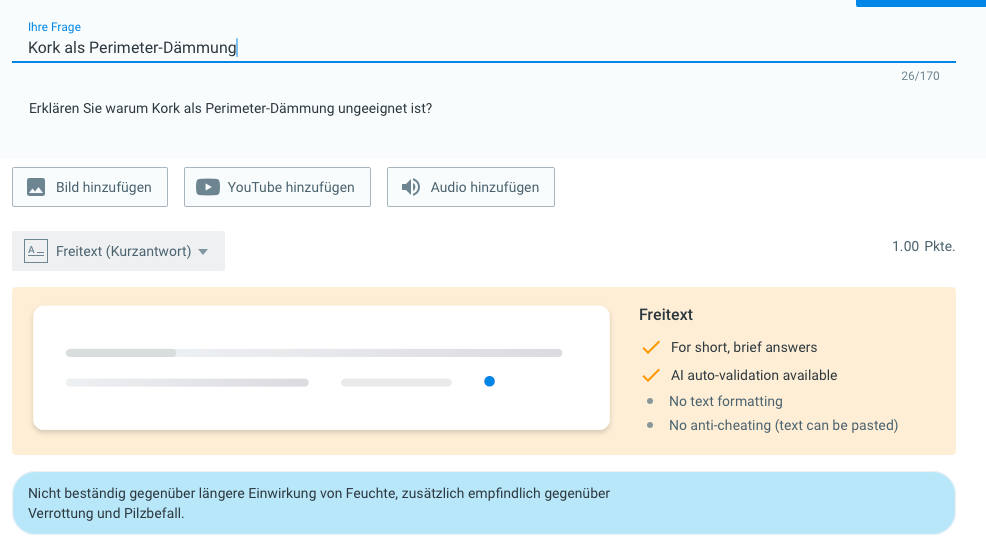
\includegraphics[width=0.7\linewidth]{Bilder/Bsp_Freitextfrage.png}
    \caption{Beispiel einer Prüfungsfrage mit Freitext.}
    \label{fig:bsp_Pruefung_freitext}
\end{figure}






Die schriftlich digitale Prüfungsform erlaubt auch Prüfungsfragen mit Bildern, welche die praktische Anwendung im Berufsalltag überprüfen (vgl. \cref{fig:bsp_Pruefung}).

\begin{figure}[h!bt]
	\centering
	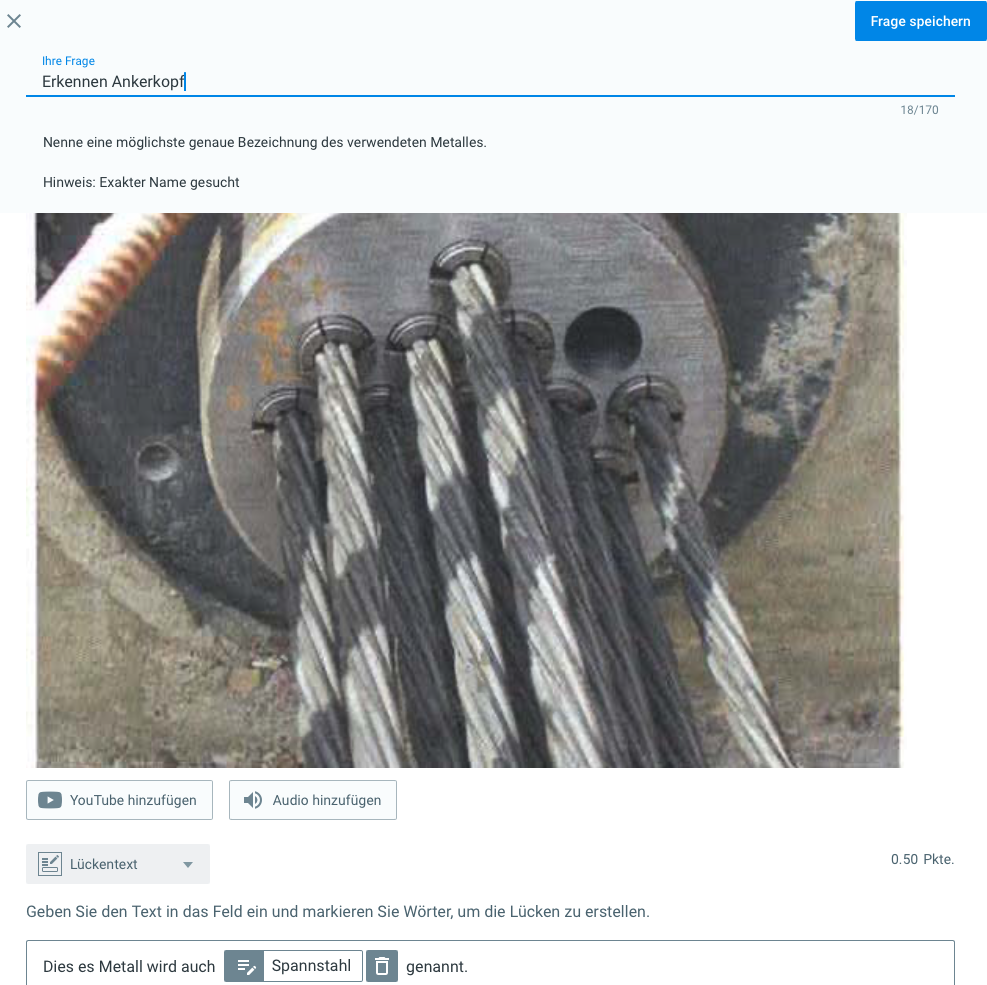
\includegraphics[width=0.7\linewidth]{Bilder/Beispiel_Anker.png}
	\caption{Beispiel einer Prüfungsfrage.}
	\label{fig:bsp_Pruefung}
\end{figure}

\FloatBarrier

Die Methodenwahl bei der Überprüfung der erworbenen Kompetenzen im Fach Baustoffe berücksichtigt damit die Lernziele des Berufspädagogischen Konzepts der BSA aktiv. Während den Prüfungen konnte:
\begin{itemize}
    \item die erworbenen Kompetenzen individuell gesammelt und dokumentiert werden.
    \item das Verstehen der erworbenen Kompetenzen gezeigt und zusammengeführt werden.
    \item die erworbenen Kompetenzen innerhalb der Prüfungsfragen angewendet angewendet, reflektiert und  diskutiert werden.
\end{itemize} 

Die Leistungsüberprüfung findet in Form einer Online­Prüfung mit dem Tool Classtime (vgl. \Cref{tab:digitales_medium}) statt. Die Prüfung umfasst Multiple-Choice­Fragen, offene Fragen und Anwendungsbeispiele zu den Schwerpunkten. Die Studierenden sollen mit der Onlineprüfung ihre Kompetenzen am Computer unter Beweis stellen. Die Prüfung wird in der Regel am Ende eines Themenblocks durchgeführt, mit einem zweiwöchigen Vorlauf zur individuellen Vorbereitung der Studierenden. Die Prüfung ist so konzipiert, dass die Studierenden die Kompetenzen der Kognitiven Taxonomiestufen K2 bis K6 nach Bloom erbringen müssen \cite{bloom1956taxonomy}. K2 können durch Multiple­Choice­Fragen abgefragt oder Zuordnungsfragen werden, während Fragen der Taxonomiestufen K3 bis K6 offene Fragen und Anwendungsbeispiele erfordern.

\subsection{Mikroebene}
Nachfolgend wird «die Feinplanung eines kleinen Ausschnitts” aus dem Lehrkonzept (vgl. \cite{Leitfaden_Aufgabenstellung_Lehrkonzept}) detailliert mit eigenen Überlegungen dargelegt. Das gesamte Lehrkonzept “Betonn” umfasst die Lektionen: 

\begin{itemize}[leftmargin=*, labelsep=0.5cm]
    \item \textbf{Lektion 1 und 2:} Einführung in Beton
    \item \textbf{Lektion 3 und 4:} Kornzusammensetzung, Korngrößenverteilung und Zusatzmittel
    \item \textbf{Lektion 5 und 6:} Wasser-Zement-Wert und Stoffraumrechnung
    \item \textbf{Lektion 7 und 8:} Beton nach Eigenschaften und Frischbetonprüfungen
\end{itemize}

Die 8 Lektionen des Lehrkonzepts teilen sich auf in 4 Blöcke zu je 2 Lektionen auf.
Zur detaillierten Betrachtung des «kleinen Ausschnitts» (vgl. \cite{Leitfaden_Aufgabenstellung_Lehrkonzept})  soll nachfolgend Lektion 1 und 2 «Einführung Beton» dienen. 

\section{Lernziele und –inhalte: Didaktische Analyse}
\label{sec:Lernziele}
Nachfolgend werden die Lernziele und -inhalte für den Ausschnitt Lektion 1 und 2 «Einführung Beton» aus dem Lehrkonzept betrachtet. Zudem werden die Lerninhalte mittels Sachanalyse und didaktischer Reduktion eingegrenzt und deren zeitliche Erreichung dargelegt. Die Lerninhalte werden in sinnvolle Lerneinheiten strukturiert und in Phasen des Selbst- und Kontaktstudiums eingeteilt.   


\subsection{Lernziele}
Zum allgemeinen Verständnis definiert die BSA Lernen als "einen aktiven, sozial kooperativen, individuellen Prozess, welcher durch variable Situationen angeregt und gefördert wird. Lernen im handlungskompetenzorientierten Unterricht:
\begin{itemize}
    \item wird begünstigt durch die vielfältigen und heterogenen Lerngemeinschaften und Umgebungen, aus denen unsere Studierenden kommen;
    \item legt Wert auf vielfältige Sozialformen;
    \item beinhaltet Üben und Festigen;
    \item bedeutet Sammeln, Dokumentieren, Verstehen, Analysieren, Zusammenführen, Anwenden, Diskutieren;
    \item reflektiert verschiedene Lerninhalte während der Ausbildung."
\end{itemize}

Lernen und Lehren sind miteinander verwoben. Die BSA versteht Lehren «ebenfalls als einen aktiven, sozial kooperativen, individuellen Prozess, welcher aber im Gegensatz zum Lernen dieses in verschiedenen Situationen ermöglicht (z. B. geführter Unterricht), begleitet (z. B. gecoachte Anwendungsübungen im Unterricht) und steuert (z. B. Definition vernetzter Problemstellungen in einer umfangreichen Projektarbeit). Lehren im handlungskompetenzorientierten Unterricht:
\begin{itemize}
    \item berücksichtigt das Potential aller Studierenden;
    \item vermittelt nicht nur Inhalte, sondern entwickelt auch Werte und Erwartungen;
    \item fördert und gestaltet Lernbeziehungen aktiv;
    \item anerkennt die Studierenden als Personen auf gleicher Augenhöhe.»
\end{itemize}

Diese Definitionen dienen den der Lektion zugrunde liegenden Lernzielen als wichtige und handlungsorientierende Grundlage. Hierbei reichtet die BSA «ihr gesamtes Handeln an folgenden vier Prinzipien aus~\cite{BerufspädagogischesKonzept_BauschuleAarau}:
\begin{enumerate}
    \item \textbf{Bildet} Fachkräfte für die Praxis aus.
    \item \textbf{Unterstützt} und entwickelt Persönlichkeiten für die Baubranche.
    \item \textbf{Macht} Lernerlebnisse erlebbar.
    \item \textbf{Realisiert} handlungsorientiertes Lernen.
\end{enumerate}

Diese vier Prinzipien dienen den Lernzielen als Kompass und beschreiben, worauf die Lernziele im Grunde abzielen, nämlich für die Praxis ausgebildete, pro-aktive und teamfähige Persönlichkeiten auszubilden, die mit realitätsnahen und brauchbaren Lernmethoden unterrichtet wurden. Auch diese Prinzipien fliessen in die der Lektion zugrunde liegenden Lernziele mit ein.

Neben den Prinzipien, Definitionen und Werten der Bauschule Aarau, richten sich die Lernziele auch an den Kognitive Taxomoniestufen nach Bloom \cite{bloom1956taxonomy} aus:


\begin{table}[H]
    \centering
    \caption{Kognitive Taxonomiestufen nach Bloom \cite{bloom1956taxonomy}, adaptiert von \cite{BerufspädagogischesKonzept_BauschuleAarau}.}
    \begin{longtable}{@{}llp{12.5cm}@{}}
        \toprule
        \textbf{Stufe} & \textbf{Begriff} & \textbf{Beschreibung}                                                                                                                                                    \\
        \midrule
        K1              & Wissen           & Sie geben gelerntes Wissen wieder und rufen es in gleichartiger Situation ab.                                                                                            \\
        K2              & Verstehen        & Sie erklären oder beschreiben gelerntes Wissen in eigenen Worten.                                                                                                        \\
        K3              & Anwenden         & Sie wenden gelernte Technologien/Fertigkeiten in unterschiedlichen Situationen an.                                                                                       \\
        K4              & Analyse          & Sie analysieren eine komplexe Situation, d.h. sie gliedern Sachverhalte in Einzelelemente, decken Beziehungen zwischen Elementen auf und finden Strukturmerkmale heraus. \\
        K5              & Synthese         & Sie kombinieren einzelne Elemente eines Sachverhalts und fügen sie zu einem Ganzen zusammen.                                                                             \\
        K6              & Beurteilen       & Sie beurteilen einen mehr oder weniger komplexen Sachverhalt aufgrund von bestimmten Kriterien.                                                                          \\
        \bottomrule
    \end{longtable}
    \label{tab:Bloom}
\end{table}

Die \Cref{tab:Bloom} genannten und definierten Begriffe sind unerlässlich, um die Lernziele für den Unterricht zu operationalisieren und zu «Lernerlebnissen» (s. o.) zu machen.

Daraus lassen sich folgende, übergeordnete Lernziele \cite{Lernfeldkatalog_Baufuehrer} für die Lektionen 1 bis 8 ableiten:
\begin{itemize}
    \item Bauführer/innen informieren sich über neue Methoden und Technologien und den Einsatz von multifunktionalen und intelligenten Baustoffen in ihrem Arbeitsbereich.
    \begin{itemize}
        \item Sie informieren sich aus Fachpresse und Messen über Innovationen. (K2)
        \item Sie betreiben ein firmeninternes Wissensmanagement zukunftsorientiert. (K4)
        \item Sie erarbeiten Dokumentationen zur Einführung von kreislauffähigen Materialien und Baumethoden in ihrem Bereich. (K4)
    \end{itemize}
    \item Bauführer und Bauführerinnen leiten den fachgerechten und vorschriftsmässigen Einsatz neuer Methoden, Technologien und Baustoffe.
    \begin{itemize}
        \item Sie wenden neue Methoden, Technologien und Baustoffe bei Bauarbeiten an. (K3)
        \item Sie instruieren die Mitarbeitenden in neuen Bauabläufen. (K3)
        \item Sie führen Evaluationen zum Einsatz von neuen Baustoffen durch. (K4)
    \end{itemize}
\end{itemize}

Die aktiven und beobachtbaren Lernziele für den «kleinen Ausschnitt» (siehe (vgl. \cite{Leitfaden_Aufgabenstellung_Lehrkonzept}) der Lektion 1 und 2 «Einführung Beton» lauten, unter Berücksichtigung der o. g. Ausführungen, wie folgt: 

\begin{itemize}
    \item \textcolor{blue}{Die Studierenden kennen die wichtigsten Bestandteile von Beton definieren und benennen.}
    \item \textcolor{blue}{Die Studierenden können die wichtigsten historischen Meilensteine der Entwicklung des Betons aufzählen.}
    \item \textcolor{blue}{Die Studierenden können die wichtigsten Unterschiede bezüglich Zusammensetzung und Eigenschaften zwischen Beton, Mörtel und Zementleim differenzieren.}
    \item \textcolor{blue}{Die Studierenden kennen die wichtigsten Eigenschaften von Gesteinskörnungen im Beton und können diese klassifizieren.}
\end{itemize}

\subsubsection{Lerninhalte}
Die Lerninhalte der Lektionen orientieren sich an dem RITA­Modell, wodurch gewährleistet wird, dass die o. g. Lernziele erreicht werden. Bei dem RITA-Modell werden die Studierenden in den Lektionen mit konkreten Aufgaben aus der Praxis konfrontiert und ihr Vorwissen, ihre Erfahrungen, Haltungen zum Thema oder gar erste Problemlösungen werden aktiviert. Dieser rhythmisierte Unterrichtsablauf wird in \cref{tab:RITA_Modell} dargestellt und ist Teil des berufspädagogischen Konzepts der BSA \cite{BerufspädagogischesKonzept_BauschuleAarau}. Hierbei liegt auch die Eignung zum erfolgreichen und verantwortungsvollen beruflichen Handeln in bestimmten konkreten und für den Beruf typischen Handlungssituationen \cite{BerufspädagogischesKonzept_BauschuleAarau} im Vordergrund.


\begin{table}[H]
    \centering
    \label{tab:RITA_Modell}
    \caption{RITA-Modell, adaptiert von \cite{BerufspädagogischesKonzept_BauschuleAarau}.}
    \begin{tabularx}{\textwidth}{@{}llp{9.5cm}@{}}
        \toprule
        \textbf{Phase} & \textbf{Beschreibung}     & \textbf{Umschreibung}                                                                                                                                               \\
        \midrule
        R:             & Ressourcen aktivieren     & Studierende werden mit konkreten Aufgaben aus der Praxis konfrontiert; Vorwissen, Erfahrungen, Haltungen zum Thema oder gar erste Problemlösungen werden aktiviert. \\
        I:             & Informationen verarbeiten & {}                                                                                                                                                                  \\
        T:             & Transfer anbahnen         & {}                                                                                                                                                                  \\
        A:             & Auswerten                 & {}                                                                                                                                                                  \\
        \bottomrule
    \end{tabularx}
\end{table}

\subsubsection{Sachanalyse und didaktische Reduktion}
\label{sssec:Sachanalyse}
Die Sachanalyse zum Thema \textbf{Beton} im Fach Baustoffe umfasst die folgenden zentralen Aspekte, die in den 8 Lektionen behandelt werden könnten:

\begin{itemize}
    \item Definition neuer Baustoffe:
          \begin{itemize}
              \item Materialien mit verbesserten Eigenschaften (langlebiger, schneller befahrbar) oder neuen Anwendungsmöglichkeiten im Hoch- oder Tiefbau.
              \item Kombination von traditionellen und innovativen Materialien (z.B. Bei der Sanierung)
          \end{itemize}
    \item Bedeutung für die Bauindustrie:
          \begin{itemize}
              \item Beitrag zur Nachhaltigkeit und Energieeffizienz.
              \item Anpassung an neue Bauweisen und technologische Anforderungen.
              \item Erfüllung von Kundenanforderungen und aktuellen Trends (z.B. ökologische Bauweise)
          \end{itemize}
\end{itemize}

\paragraph{Eigenschaften und Kategorien neuer Baustoffe}
\begin{itemize}
    \item \textbf{Verbesserte Eigenschaften:}
          \begin{itemize}
              \item Höhere Festigkeit und Stabilität durch unterschiedliche strukturen auf unterschiedlichen Grössenskalen.
              \item Geringeres Gewicht bei gleicher Tragfähigkeit.
              \item Verbesserte Isolations- und Dämmeigenschaften.
          \end{itemize}
    \item \textbf{Kategorien:}
          \begin{itemize}
              \item Hochleistungsbeton (z. B. UHPC - Ultra High Performance Concrete).
              \item Selbstheilender Beton.
              \item Nanomaterialien (z. B. Nanobeschichtungen, Nanopartikel in Beton).
              \item Recycling-Baustoffe (z. B. Sekundärrohstoffe aus Abbruchmaterialien).
              \item Neuartige Baustoffe (z. B. Carbonbeton, usw.).
          \end{itemize}
\end{itemize}

\paragraph{Technologien zur Herstellung und Verarbeitung}
\begin{itemize}
    \item Additive Fertigung:
          \begin{itemize}
              \item 3D-Druck von Beton und anderen Baustoffen.
          \end{itemize}
    \item Digitalisierung im Bauwesen:
          \begin{itemize}
              \item Building Information Modeling (BIM) zur Optimierung der Materialauswahl.
              \item Einsatz von Drohnen zur Baustoffüberwachung oder des Baufortschrittes
              \item Softwarelösungen zur Materialplanung und -kontrolle.
          \end{itemize}
    \item Modulares Bauen:
          \begin{itemize}
              \item Baustoffe für vorgefertigte Bauelemente.
              \item Effizienzsteigerung durch modulare Konstruktion.
          \end{itemize}
\end{itemize}

\paragraph{Nachhaltigkeit und Umweltverträglichkeit}
\begin{itemize}
    \item Reduktion des ökologischen Fussabdrucks:
          \begin{itemize}
              \item Nutzung von Recyclingmaterialien in Projekten.
              \item Energieeffiziente Produktionsverfahren oder Baumaschinen.
          \end{itemize}
    \item Lebenszyklusanalyse:
          \begin{itemize}
              \item Bewertung der Umweltbelastung über die gesamte Lebensdauer.
          \end{itemize}
    \item Kreislaufwirtschaft im Bauwesen:
          \begin{itemize}
              \item Wiederverwendbare und recycelbare Baustoffe.
              \item Reduktion von Abfall durch geschlossene Materialkreisläufe.
          \end{itemize}
    \item Nachhaltigkeitszertifikate:
          \begin{itemize}
              \item Green Building Labels (z. B. LEED, Minergie).
              \item Bewertung durch Ökobilanzen (z. B. graue Energie, CO2-Fussabdruck).
              \item Einhaltung von Umweltstandards und -richtlinien.
              \item Minergie, Minergie-P, Minergie-A, Minergie-Eco, Minergie-Modul, Minergie-ECO-P, Minergie-ECO-A, Minergie-ECO-Modul, Minergie-ECO-Modul-P, Minergie-ECO-Modul-A Standards
          \end{itemize}
\end{itemize}

\paragraph{Herausforderungen und Potenziale}
\begin{itemize}
    \item Herausforderungen:
          \begin{itemize}
              \item Hohe Kosten und aufwendige Produktionsverfahren.
              \item Akzeptanz bei Bauunternehmen und Bauherren.
              \item Anforderungen an die Lagerung und Logistik (z. B. Feuchtigkeitsschutz).
          \end{itemize}
    \item Potenziale:
          \begin{itemize}
              \item Verbesserung der Bauqualität und -geschwindigkeit.
              \item Beitrag zu nachhaltigem und energieeffizientem Bauen.
              \item Langlebigkeit und Wartungsfreundlichkeit der Baustoffe resp. der Bauwerke
          \end{itemize}
\end{itemize}

\paragraph{Schadensfälle im Bauwesen und deren Vermeidung}
\begin{itemize}
    \item Häufige Schadensfälle durch ungeeignete oder fehlerhafte Baustoffe:
          \begin{itemize}
              \item Korrosion von Stahl  (chlorid- oder carbonatisierungbedingt) in Beton.
              \item Frostschäden bei Beton.
          \end{itemize}
    \item Massnahmen zur Vermeidung:
          \begin{itemize}
              \item Auswahl geeigneter Baustoffe für spezifische Umweltbedingungen.
              \item Regelmässige Materialprüfungen und Qualitätskontrollen.
              \item Schulung von Mitarbeitenden im Umgang mit neuen Materialien.
          \end{itemize}
\end{itemize}

\paragraph{Anwendungsbeispiele}
\begin{itemize}
    \item Selbstheilender Beton in Infrastrukturbauten (z. B. Brücken, Tunnel).
    \item 3D-gedruckte Gebäude zur Reduktion von Bauzeit und -kosten.
    \item Einsatz von Recyclingbeton in Neubauten und Renovierungsprojekten.
    \item Einsatz von Nanomaterialien zur Verbesserung der Oberflächeneigenschaften von Fassaden.
    \item Verwendung von Carbonbeton für leichtere und langlebigere Bauwerke.
    \item Integration von Photovoltaik in Baumaterialien zur Energiegewinnung.
    \item Verwendung von recyceltem Kunststoff in Asphaltmischungen für Strassenbau.
    \item Anwendung von Hochleistungsbeton in Hochhäusern und Brücken.
    \item Nutzung von 3D-gedruckten Bauteilen für schnelle und kosteneffiziente Bauprojekte.
    \item Einsatz von intelligenten Baustoffen mit Sensoren zur Überwachung der Bauwerksintegrität.
\end{itemize}


\paragraph{Fazit:} Aus der Sachanalyse haben sich die folgenden Lektionen (Doppelstunden) ergeben, welche Lerninhalte und Lernziele optimal miteinander kombinieren und abdecken: 

\begin{itemize}[leftmargin=*, labelsep=0.5cm]
    \item \textbf{Lektion 1 und 2:} Einführung in Beton
    \item \textbf{Lektion 3 und 4:} Kornzusammensetzung, Korngrößenverteilung und Zusatzmittel
    \item \textbf{Lektion 5 und 6:} Wasser-Zement-Wert und Stoffraumrechnung
    \item \textbf{Lektion 7 und 8:} Beton nach Eigenschaften und Frischbetonprüfungen
\end{itemize}


\subsection{Zeitliche Einteilung des Lehrkonzepts}
\label{sssec:ZeitlicheEinteilungLK}
Die aus der Sachanalyse gewonnen Lerninhalte und Lernziele (vgl. \Cref{sssec:Sachanalyse}) können in der zur Verfügung stehenden Zeit wie in \Cref{tab:lektionen_beton} dargestellt aufgeteilt werden. Dabei wird für jede Doppelstunde ein Schwerpunkt gesetzt, der in der jeweiligen Lektion behandelt wird. Die Lektionen bauen aufeinander auf.
\begin{table}[H]
    \centering
    \caption{Übersicht der Lektionen zum Lehrkonzept Beton}
    \begin{tabularx}{\linewidth}{@{}lX@{}}
        \toprule
        \textbf{Datum} & \textbf{Lektionen} \\
        \midrule
        03.02.2025 & \textbf{Lektion 1 und 2:} Einführung in Beton \\
        \addlinespace
        10.02.2025 & \textbf{Lektion 3 und 4:} Kornzusammensetzung und Zusatzmittel \\
        \addlinespace
        17.02.2025 & \textbf{Lektion 5 und 6:} Wasser-Zement-Wert und Stoffraumrechnung \\
        \addlinespace
        24.02.2025 & \textbf{Lektion 7 und 8:} Beton nach Eigenschaften und Frischbetonprüfungen \\
        \bottomrule
    \end{tabularx}
    \label{tab:lektionen_beton}
\end{table}

\subsection{Struktur der Lerneinheiten}
Die Struktur der Lerneinheiten umfasst, angelehnt an das Kompetenzprofil der Bauführer und Bauführerinnen \cite{Kompetenzprofil_Baufuehrer}, das Berufspädagogische Konzept der BSA \cite{BerufspädagogischesKonzept_BauschuleAarau} und den Lernfeldkatalog Bauführer/in HFP \cite{Lernfeldkatalog_Baufuehrer}, aktive Unterrichtseinheiten und theoretische Einheiten während der Lektionen. Hierbei sind stets die allgemein definierten Lern- und Lehrziele (s. o.) Grundlage bei der Erarbeitung der Unterrichtsstruktur. Jede Lektion wird individuell nach Thema ausgearbeitet und auch während der Lektionen soll genügend Raum für spontane Nachfragen und/oder Diskussionen zu den behandelten Themen während der Lerneinheit durch die LP geboten werden. Eine Grundstruktur der Lerneinheiten beinhaltet, unter Berücksichtigung aller o. g. Ausführungen: 

\begin{itemize}
    \item[\textrightarrow] Begrüßung mit interaktivem Einstieg in die Lektion (z. B. Blitzlicht)
    \item[\textrightarrow] Übersichtsfolie zum Ablauf der Lektion (inkl. zeitlichem und inhaltlichem Überblick)
    \item[\textrightarrow] Übersichtsfolie zu den Lernzielen der Lektion (zur Orientierung für die Studierenden und zur Leistungskontrolle)
    \item[\textrightarrow] Theoretische Einheiten (zur Wissensvermittlung)
    \item[\textrightarrow] Praktische Einheiten (zur Förderung des Austauschs, der Sozialkompetenzen und Aktivierung des Wissens)
    \item[\textrightarrow] Leistungsüberprüfung (z. B. in Form eines digitalen Quiz zum Abschluss der Lektion)
\end{itemize}
Diese Elemente einer Lerneinheit orientieren sich in der Sturktur an dem jeweiligen Thema und den Bedürfnissen der Studierenden zu dem spezifischen Thema. 


Für die Lektionen 1 und 2 «Einführung Beton» könnte ein Auszug aus der Lektion wie in \Cref{tab:ablauf_beton} dargestellt aussehen. Dabei wird auf die Methodeneinsätze und die Sozialformen eingegangen, die in der jeweiligen Lektion zum Einsatz kommen.
Die Detailplanung befindet sich im Anhang (siehe \Cref{ssec:Beton_Einführung_Folien}).
\begin{table}[h!tb]
    \centering
    \caption{Ablauf und Methodeneinsatz für die Lektion Beton}
    \begin{tabularx}{\textwidth}{@{}p{2.9cm}p{6.4cm}X@{}}
        \toprule
        \textbf{Uhrzeit} & \textbf{Ablauf} & \textbf{Methodeneinsatz und Sozialform} \\
        \midrule
        15:15 -- 15:30 Uhr & Einführung in das Thema Beton & Blitzlicht \\
        15:30 -- 16:00 Uhr & Abgrenzung zw. Beton und Mörtel & Mentimeter: Multiple-Choice, offene und halboffene Fragen \\
        16:00 -- 16:10 Uhr & Pause & -- \\
        16:10 -- 16:25 Uhr & Wichtigkeit der Gesteinskörnung im Beton & Gruppenarbeit \\
        16:25 -- 16:35 Uhr & Einführung Lernwerkstatt und Abschluss der Lektion & Einzelarbeit \\
        16:35 -- 17:00 Uhr & Arbeit an Lernwerkstatt & Einzelarbeit \\
        \bottomrule
    \end{tabularx}
    \label{tab:ablauf_beton}
\end{table}
\FloatBarrier
\subsection{Einteilung Selbst- und Kontaktstudium}
Die 8 Lektionen finden im Kontaktstudium statt. Während des Kontaktstudiums sollen die Lerninhalte und -ziele vermittelt werden (s. o.). Im Anschluss an das Kontaktstudium, sprich nach jeder Doppellektion (z. B. im Anschluss an die Lektionen 1 und 2 «Einführung Beton») folgt das Selbststudium der Studierenden bei sich Zuhause.

Innerhalb des Selbststudiums sollen die Kompetenzen der angehenden Bauführer und Bauführerinnen zur Selbstorganisation gefördert werden. Zudem sollen die Lerninhalte aus dem Kontaktstudium vertieft und überprüft werden. 

Daraus ergibt sich für die 8 Lektionen eine immer wiederkehrende Verknüpfung (vgl. \Cref{fig:Zyklus_Selbst_Kontaktstudium}) von Selbst- und Kontaktstudium.

\begin{figure}[h!bt]
	\centering
    \begin{tikzpicture}[node distance=0.50cm, auto]

        % Position der Blöcke
        \node [block] (kontakt1) {Kontaktstudium \\ (à 2 Lektionen)};
        \node [block, below right of=kontakt1, xshift=2.5cm, yshift=-1cm] (selbst1) {Selbststudium};
        \node [block, below left of=selbst1, xshift=-2.5cm, yshift=-1cm] (kontakt2) {Kontaktstudium \\ (à 2 Lektionen)};
        \node [block, above left of=kontakt2, xshift=-2.5cm, yshift=1cm] (selbst2) {Selbststudium};

        % Pfeile zwischen den Blöcken
        \draw [arrow] (kontakt1) -- (selbst1);
        \draw [arrow] (selbst1) -- (kontakt2);
        \draw [arrow] (kontakt2) -- (selbst2);
        \draw [arrow] (selbst2) -- (kontakt1);

    \end{tikzpicture}
	\caption{Phase des Selbst- und Kontaktstudiums im Lehrkonzept.}
	\label{fig:Zyklus_Selbst_Kontaktstudium}
\end{figure}

Diese Repetition aus Wissensvermittlung und Wiederholen des Gelernten ist unerlässlich für ein aktives Verständnis der Lerninhalte und die Ausbildung konkreter Verständnisfragen im Fach Baustoffe. 

\subsection{Methoden und Aufträge}

Der im Fachkurs behandelte Methodenpool gibt spannende Anregungen für die Anwendung unterschiedlicher Methoden innerhalb der 8 Lerneinheiten zum Thema «Beton» \cite{unikoelnMethodenpool}. An dem Methodenpool wurde sich auch bei der Ausgestaltung der Lektionen 1 und 2 «Einführung Beton» im Hinblick auf die sinnvolle Anwendung unterschiedlicher Methoden orientiert. 

Gerade um das Kontaktstudium zum «Lernerlebnis» \cite{BerufspädagogischesKonzept_BauschuleAarau} zu machen, ist eine Methodenvielfalt bei den 8 Lektionen angebracht. 
Beispielhaft wurde bereits Lektion 1 «Einführung Beton» angeführt in \Cref{tab:lektionen_beton}.

Man erkennt den Einsatz des Blitzlichts als Methode: gerade zu Beginn einer Lektion kann das Blitzlicht als Icebreaker dienen und die Stimmung und Aufmerksamkeit der Studierenden einfangen. 
Um die Aktivierung und auch digitale Kompetenz der Studierenden zu fördern, kommt im Laufe der Lektion die Applikation Mentimeter zum Einsatz. Hier werden die Studierenden durch Multiple-choice, offene und halb-offene Fragen zur aktiven Teilnahme am Unterrichtsgeschehen angeregt, das Thema wird gamifiziert und den Studierenden auf spielerische Weise nochmals nahegebracht. 

Bei dem Methodeneinsatz der Gruppenarbeit werden die Sozialkompetenzen der angehenden Bauführer und Bauführerinnen gefördert. Wie unter 1.2 Zielgruppe ersichtlich, ist die Teamarbeit für die Zielgruppe in ihrer Praxistätigkeit unerlässlich und gehört zu ihren täglichen Herausforderungen. Daher ist diese Methode von grosser Bedeutung innerhalb der Lektionen im Fach Baustoffe. 

Die Methode der Lernwerkstatt lässt unterschiedliche Arbeitsaufträge zu: so können die Studierenden sich in einem anderen Raum ein Bild von den innerhalb der Lektion besprochenen Gesteinen machen, diese beschreiben und definieren, was die Praxiserfahrung ins Zentrum stellt. Die Bearbeitung eines digitalen Quiz in Einzelarbeit hilft bei der Überprüfung der erreichten Lernziele. Hierbei erfolgt auch eine direkte Rückmeldung durch die LP: die LP hat Einblick in die Bearbeitung und Ergebnisse des Quiz und kann den Studierenden hier individuell Rückmeldung zu ihren Lernergebnissen geben. Hierdurch hat die LP auch einen Überblick über den Leistungsstand der Studierenden und kann die Methoden für die kommende Lektion entsprechend anpassen, da sie die Bedürfnisse der Studierenden kennt. 

Für das Selbststudium kommt vorwiegend eine digitale Methode zum Einsatz: die Applikation MS Teams. Innerhalb dieser Applikation erhalten die Studierenden ihre Aufträge durch die LP. Die Aufträge für das Selbststudium umfassen das dort abgelegte Unterrichtsskript, die Folien zu den Lektionen und ergänzende schriftliche Übungen (z. B. Berechnungsaufgaben). Die Aufträge innerhalb des Selbststudiums zielen auf die Selbstorganisation und intrinsische Motivation der Studierenden ab, da vor allem die Übungen meist freiwillig sind und als Vertiefung und Ergänzung dienen. 

\subsection{ Learning Management System (MS Teams)}
\label{sssec:MS_Teams_LMS}

Der MS-Teams-Kanal wird jeweils vom Sekretariat spezifisch für jede Klasse vorbereitet. Der Kanal wird nach der Klasse benannt und weiterunterteilt nach Fächern (z.B. Baustoffe). Im Fach Baustoffe wird der Kanal nochmals unterteilt in die unterschiedlichen Baustoffe, zusätzlich gibt es einen Allgemeinen Teil. Die Unterlagen zu den unterschiedlichen Baustoffen werden in der Regel als eine Präsentation hochgeladen. Die Aufträge jeweils vor den Unterrichtslektionen und die Lösungen nach dem Abschluss der Aufgabe nach der Lektion. Im Allgemeinen Teil wird jeweils spezifische Vorbereitungen auf die Prüfungen abgelegt, dies jeweils spätestens 2 Wochen vor dem Prüfungstermin. Die einzelnen Fächer sind in der Regel nochmals weiter unterteilt in 01\_Slides, 02\_Aufgaben und 03\_Lösungen.  

Über Assignments in MS-Teams werden unterschiedliche Aufträge an die Studierenden verteilt. Sobald der Auftrag verteilt wird, wird im Reiter Posts eine Notiz erstellt und die Studierenden werden gleichzeitig über eine Aktivität über den Auftrag informiert. Je nach Art des Assignments werden den Studierenden Feedback über eine automatische Korrektur  gegeben (Anzahl erreichter Punkte) oder bestanden resp. nicht bestanden. 
Die Studierenden kommunizieren untereinander über MS-Teams in privaten Chats, jedoch nicht im Kanal Baustoffe. MS-Teams dient ebenfalls der Kommunikation zwischen LP und den Studierenden. Beispielsweise erfolgt die Rückgabe der Prüfung inkl. Note über private Chats mit der LP. 

Dem Coach wurde Zugriff auf dem Teams-Kanal Baustoffe erteilt.

\subsection{Gender- und diversitygerechte Lehre}
Die Umsetzung einer gender- und diversitygerechten Lehre orientiert sich an drei zentralen Komponenten: Vermittlung, Aktivierung und Begleitung, wie in der didaktischen Pyramide nach Reinmann (2015) dargestellt. Diese Komponenten tragen gemeinsam dazu bei, eine inklusive und wertschätzende Lernumgebung zu schaffen, die die individuellen Bedürfnisse und Hintergründe der Studierenden berücksichtigt und als fair und motivierend für alle Studierenden wahrgenommen wird.

Bei der Vermittlung der Inhalte wird darauf geachtet, dass Beispiele und Fallstudien aus verschiedenen Perspektiven gewählt werden, um unterschiedliche Lebensrealitäten und berufliche Erfahrungen abzubilden. So werden in den Lektionen zur Materialkunde etwa sowohl klassische Baustoffe als auch innovative und nachhaltige Materialien behandelt, deren Einsatzmöglichkeiten vielfältige Anforderungen abdecken. Zudem kommen Lehrmaterialien zum Einsatz, die geschlechtergerecht formuliert sind, um alle Studierenden gleichermassen anzusprechen.

Die Aktivierung erfolgt durch vielfältige Methoden wie Gruppenarbeiten, interaktive Tools oder gemeinsame Diskussionen. Ein Beispiel aus der Praxis sind digitale Umfragen mit Mentimeter, die es allen Studierenden ermöglichen, ihre Meinungen und Vorkenntnisse aktiv einzubringen. In Gruppenarbeiten wird darauf geachtet, Teams heterogen zu besetzen, damit die Studierenden voneinander lernen und unterschiedliche Sichtweisen einbringen können. Dies fördert sowohl die aktive Auseinandersetzung mit dem Thema als auch die Sozialkompetenz, die für die spätere Tätigkeit als Bauführer und Bauführerin entscheidend ist.

Die Begleitung der Studierenden wird durch regelmässige Feedbackgespräche und den Einsatz von digitalen Plattformen wie MS Teams unterstützt. Die LP stellt sicher, dass alle Lernmaterialien gut strukturiert und frühzeitig zur Verfügung stehen, um den Studierenden eine effektive Vorbereitung zu ermöglichen. Individuelle Rückmeldungen, z. B. nach digital durchgeführten Tests, bieten Gelegenheit zur Förderung und Unterstützung, insbesondere für die Studierenden mit unterschiedlichen Vorkenntnissen. 

Durch diese praxisnahe Umsetzung wird eine Lernumgebung geschaffen, die sowohl die Vielfalt der Studierenden wertschätzt als auch ihre individuellen Potenziale fördert.

\clearpage




\clearpage
\addcontentsline{toc}{section}{Quellenangaben}

\printbibliography

\clearpage
\appendix
\section{Anhang}
\subsection{Beton Einführung}
\label{ssec:Beton_Einführung_Folien}
\textcolor{blue}{Hier kommen noch die Folien.}
%\subsection{Lernziele}
%\subsubsection*{Beton}
Die Studierenden: 

\begin{itemize}[noitemsep]
	%\item kennen Frisch- und Festbetonprüfungen mit den Druckfestigkeitsklassifikation beschreiben.
	\item kennen die Ausgangsstoffe von Beton und können eine Mischungsberechnung (Stoffraumrechnung) durchführen
	%\item können Ziel- und Steuergrössen festlegen 
	\item können für übliche Praxisanwendungen die entsprechende Betonfestlegung bestimmen.
	\item kennen die Geschichte des Betons. 
	\item kennen mögliche Definition von Beton (z.B. nach SIA 262), sowie dessen Bestandteile.
	\item können die Unterschiede zwischen Beton und Mörteln resp. Bindemitteln erläutern. 
	\item kennen die Vorteile von Gesteinskörungen bei der Herstellung von Beton, sowie dessen Auswirkungen bezügliche den Frisch- und Festbetoneigenschaften.
	\item kennen die Eigenschaften der Gesteinskörnung, die Wichtigkeit der Siebkurve (maximale Packung und Grössenverteilung) (inkl. der Auswirkungen auf die Eigenschaften von Frisch- und Festbeton).
	\item können Gesteinskörungen nach unterschiedlichen Eigenschaften klassifizieren (z.B. Rohdichte). 
	\item kennen die Begriffe Mehlkorngehalt, Zugabewasser und deren Auswirkungen bei der Herstellung von Beton.
	\item kennen mindestens die folgenden Zusatzmittel und deren Auswirkungen auf die Frisch- und Festbetoneigenschaften, sowie kennen deren Funktionsweise: Betonverflüssiger, Fliessmittel, Luftporenbildner, Verzögerer, Luftporenbildner, Erstarrungs- und Erhärtungsbeschleuniger, Dichtungsmittel, Stabilisierer. 
	\item kennen Einflussfaktoren, welche die Wirksamkeit von Zusatzmittel beeinflussen können, sowohl positiv wie auch negativ.
	\item kennen die Auswirkungen der Wahl des w/z-Wertes und können eigenständig Berechnungen durchführen.
	\item kennen die Entwicklung der Festigkeit von Beton über die Zeit.
	%\item kennen die Begriffe "Beton nach Zusammensetzung" und Beton nach Eigenschaften, sowie die Druckfestigkeitsklassen von Beton.
	%\item können Expositionsklassen für übliche Anwendungen bestimmen und somit auch einen geeigneten Beton selektieren.
\end{itemize}


\end{document}